%% Creator: Inkscape 0.91, www.inkscape.org
%% PDF/EPS/PS + LaTeX output extension by Johan Engelen, 2010
%% Accompanies image file 'Histogram_transformace.pdf' (pdf, eps, ps)
%%
%% To include the image in your LaTeX document, write
%%   \input{<filename>.pdf_tex}
%%  instead of
%%   \includegraphics{<filename>.pdf}
%% To scale the image, write
%%   \def\svgwidth{<desired width>}
%%   \input{<filename>.pdf_tex}
%%  instead of
%%   \includegraphics[width=<desired width>]{<filename>.pdf}
%%
%% Images with a different path to the parent latex file can
%% be accessed with the `import' package (which may need to be
%% installed) using
%%   \usepackage{import}
%% in the preamble, and then including the image with
%%   \import{<path to file>}{<filename>.pdf_tex}
%% Alternatively, one can specify
%%   \graphicspath{{<path to file>/}}
%%
%% For more information, please see info/svg-inkscape on CTAN:
%%   http://tug.ctan.org/tex-archive/info/svg-inkscape
%%
\begingroup%
  \makeatletter%
  \providecommand\color[2][]{%
    \errmessage{(Inkscape) Color is used for the text in Inkscape, but the package 'color.sty' is not loaded}%
    \renewcommand\color[2][]{}%
  }%
  \providecommand\transparent[1]{%
    \errmessage{(Inkscape) Transparency is used (non-zero) for the text in Inkscape, but the package 'transparent.sty' is not loaded}%
    \renewcommand\transparent[1]{}%
  }%
  \providecommand\rotatebox[2]{#2}%
  \ifx\svgwidth\undefined%
    \setlength{\unitlength}{412bp}%
    \ifx\svgscale\undefined%
      \relax%
    \else%
      \setlength{\unitlength}{\unitlength * \real{\svgscale}}%
    \fi%
  \else%
    \setlength{\unitlength}{\svgwidth}%
  \fi%
  \global\let\svgwidth\undefined%
  \global\let\svgscale\undefined%
  \makeatother%
  \begin{picture}(1,0.58252427)%
    \put(0.16785498,0.25961273){\color[rgb]{0,0,0}\makebox(0,0)[b]{\smash{\textbf D)}}}%
    \put(0.02144059,0.00096056){\color[rgb]{0,0,0}\makebox(0,0)[rb]{\smash{}}}%
    \put(0.2183453,0.12332277){\color[rgb]{0,0,0}\makebox(0,0)[rb]{\smash{}}}%
    \put(0.49795206,0.25961273){\color[rgb]{0,0,0}\makebox(0,0)[b]{\smash{\textbf E)}}}%
    \put(0.82804915,0.25961273){\color[rgb]{0,0,0}\makebox(0,0)[b]{\smash{\textbf F)}}}%
    \put(0.16785498,0.57029246){\color[rgb]{0,0,0}\makebox(0,0)[b]{\smash{\textbf A)}}}%
    \put(0.25083624,0.31101275){\color[rgb]{0,0,0}\makebox(0,0)[b]{\smash{\footnotesize 255}}}%
    \put(0.28037192,0.33555078){\color[rgb]{0,0,0}\makebox(0,0)[lb]{\smash{\footnotesize input}}}%
    \put(0.06654567,0.5560292){\color[rgb]{0,0,0}\makebox(0,0)[b]{\smash{\footnotesize output}}}%
    \put(0.06800645,0.31101275){\color[rgb]{0,0,0}\makebox(0,0)[b]{\smash{\footnotesize 0}}}%
    \put(0.05533799,0.5190624){\color[rgb]{0,0,0}\makebox(0,0)[rb]{\smash{\footnotesize 255}}}%
    \put(0.05519171,0.33307358){\color[rgb]{0,0,0}\makebox(0,0)[rb]{\smash{\footnotesize 0}}}%
    \put(0.49795206,0.57029246){\color[rgb]{0,0,0}\makebox(0,0)[b]{\smash{\textbf B)}}}%
    \put(0.82804915,0.57029246){\color[rgb]{0,0,0}\makebox(0,0)[b]{\smash{\textbf C)}}}%
    \put(0.7864531,0.31101275){\color[rgb]{0,0,0}\makebox(0,0)[b]{\smash{\footnotesize min}}}%
    \put(0.864123,0.31101275){\color[rgb]{0,0,0}\makebox(0,0)[b]{\smash{\footnotesize max}}}%
    \put(0.84271845,0.085437){\color[rgb]{0,0,0}\makebox(0,0)[lb]{\smash{\footnotesize $\gamma > 1$}}}%
    \put(0.78640777,0.13786407){\color[rgb]{0,0,0}\makebox(0,0)[rb]{\smash{\footnotesize $\gamma < 1$}}}%
    \put(0,0){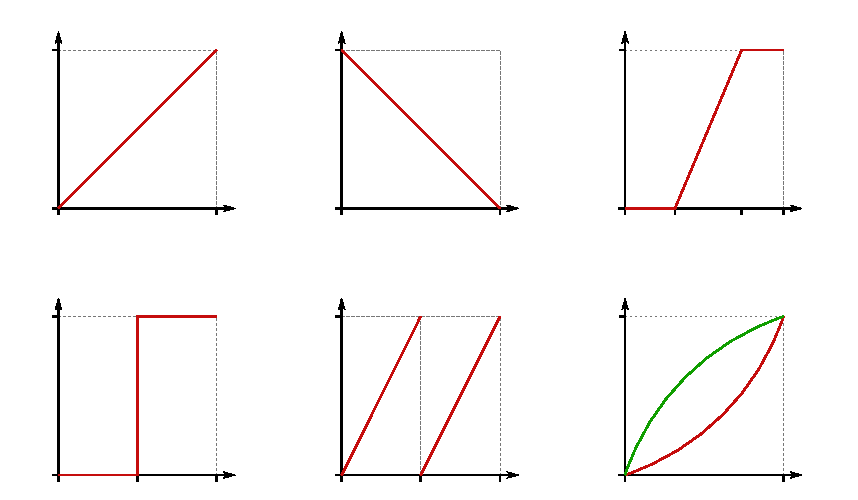
\includegraphics[width=\unitlength,page=1]{Histogram_transformace.pdf}}%
    \put(0.58093357,0.31101275){\color[rgb]{0,0,0}\makebox(0,0)[b]{\smash{\footnotesize 255}}}%
    \put(0.61046925,0.33555078){\color[rgb]{0,0,0}\makebox(0,0)[lb]{\smash{\footnotesize input}}}%
    \put(0.39664301,0.5560292){\color[rgb]{0,0,0}\makebox(0,0)[b]{\smash{\footnotesize output}}}%
    \put(0.39810379,0.31101275){\color[rgb]{0,0,0}\makebox(0,0)[b]{\smash{\footnotesize 0}}}%
    \put(0.38543532,0.5190624){\color[rgb]{0,0,0}\makebox(0,0)[rb]{\smash{\footnotesize 255}}}%
    \put(0.38528905,0.33307358){\color[rgb]{0,0,0}\makebox(0,0)[rb]{\smash{\footnotesize 0}}}%
    \put(0.91103065,0.31101275){\color[rgb]{0,0,0}\makebox(0,0)[b]{\smash{\footnotesize 255}}}%
    \put(0.94056634,0.33555078){\color[rgb]{0,0,0}\makebox(0,0)[lb]{\smash{\footnotesize input}}}%
    \put(0.72674009,0.5560292){\color[rgb]{0,0,0}\makebox(0,0)[b]{\smash{\footnotesize output}}}%
    \put(0.72820091,0.31101275){\color[rgb]{0,0,0}\makebox(0,0)[b]{\smash{\footnotesize 0}}}%
    \put(0.71553244,0.5190624){\color[rgb]{0,0,0}\makebox(0,0)[rb]{\smash{\footnotesize 255}}}%
    \put(0.71538613,0.33307358){\color[rgb]{0,0,0}\makebox(0,0)[rb]{\smash{\footnotesize 0}}}%
    \put(0.25083624,0.00033314){\color[rgb]{0,0,0}\makebox(0,0)[b]{\smash{\footnotesize 255}}}%
    \put(0.28037192,0.02487117){\color[rgb]{0,0,0}\makebox(0,0)[lb]{\smash{\footnotesize input}}}%
    \put(0.06654567,0.24534959){\color[rgb]{0,0,0}\makebox(0,0)[b]{\smash{\footnotesize output}}}%
    \put(0.06800645,0.00033314){\color[rgb]{0,0,0}\makebox(0,0)[b]{\smash{\footnotesize 0}}}%
    \put(0.05533799,0.20838279){\color[rgb]{0,0,0}\makebox(0,0)[rb]{\smash{\footnotesize 255}}}%
    \put(0.05519171,0.02239397){\color[rgb]{0,0,0}\makebox(0,0)[rb]{\smash{\footnotesize 0}}}%
    \put(0.58093357,0.00033314){\color[rgb]{0,0,0}\makebox(0,0)[b]{\smash{\footnotesize 255}}}%
    \put(0.61046925,0.02487117){\color[rgb]{0,0,0}\makebox(0,0)[lb]{\smash{\footnotesize input}}}%
    \put(0.39664301,0.24534959){\color[rgb]{0,0,0}\makebox(0,0)[b]{\smash{\footnotesize output}}}%
    \put(0.39810379,0.00033314){\color[rgb]{0,0,0}\makebox(0,0)[b]{\smash{\footnotesize 0}}}%
    \put(0.38543532,0.20838279){\color[rgb]{0,0,0}\makebox(0,0)[rb]{\smash{\footnotesize 255}}}%
    \put(0.38528905,0.02239397){\color[rgb]{0,0,0}\makebox(0,0)[rb]{\smash{\footnotesize 0}}}%
    \put(0.91103065,0.00033314){\color[rgb]{0,0,0}\makebox(0,0)[b]{\smash{\footnotesize 255}}}%
    \put(0.94056634,0.02487117){\color[rgb]{0,0,0}\makebox(0,0)[lb]{\smash{\footnotesize input}}}%
    \put(0.72674009,0.24534959){\color[rgb]{0,0,0}\makebox(0,0)[b]{\smash{\footnotesize output}}}%
    \put(0.72820091,0.00033314){\color[rgb]{0,0,0}\makebox(0,0)[b]{\smash{\footnotesize 0}}}%
    \put(0.71553244,0.20838279){\color[rgb]{0,0,0}\makebox(0,0)[rb]{\smash{\footnotesize 255}}}%
    \put(0.71538613,0.02239397){\color[rgb]{0,0,0}\makebox(0,0)[rb]{\smash{\footnotesize 0}}}%
  \end{picture}%
\endgroup%
